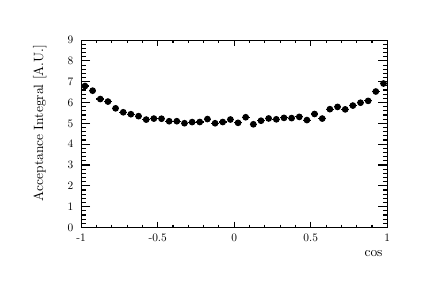
\begin{tikzpicture}
\pgfdeclareplotmark{cross} {
\pgfpathmoveto{\pgfpoint{-0.3\pgfplotmarksize}{\pgfplotmarksize}}
\pgfpathlineto{\pgfpoint{+0.3\pgfplotmarksize}{\pgfplotmarksize}}
\pgfpathlineto{\pgfpoint{+0.3\pgfplotmarksize}{0.3\pgfplotmarksize}}
\pgfpathlineto{\pgfpoint{+1\pgfplotmarksize}{0.3\pgfplotmarksize}}
\pgfpathlineto{\pgfpoint{+1\pgfplotmarksize}{-0.3\pgfplotmarksize}}
\pgfpathlineto{\pgfpoint{+0.3\pgfplotmarksize}{-0.3\pgfplotmarksize}}
\pgfpathlineto{\pgfpoint{+0.3\pgfplotmarksize}{-1.\pgfplotmarksize}}
\pgfpathlineto{\pgfpoint{-0.3\pgfplotmarksize}{-1.\pgfplotmarksize}}
\pgfpathlineto{\pgfpoint{-0.3\pgfplotmarksize}{-0.3\pgfplotmarksize}}
\pgfpathlineto{\pgfpoint{-1.\pgfplotmarksize}{-0.3\pgfplotmarksize}}
\pgfpathlineto{\pgfpoint{-1.\pgfplotmarksize}{0.3\pgfplotmarksize}}
\pgfpathlineto{\pgfpoint{-0.3\pgfplotmarksize}{0.3\pgfplotmarksize}}
\pgfpathclose
\pgfusepathqstroke
}
\pgfdeclareplotmark{cross*} {
\pgfpathmoveto{\pgfpoint{-0.3\pgfplotmarksize}{\pgfplotmarksize}}
\pgfpathlineto{\pgfpoint{+0.3\pgfplotmarksize}{\pgfplotmarksize}}
\pgfpathlineto{\pgfpoint{+0.3\pgfplotmarksize}{0.3\pgfplotmarksize}}
\pgfpathlineto{\pgfpoint{+1\pgfplotmarksize}{0.3\pgfplotmarksize}}
\pgfpathlineto{\pgfpoint{+1\pgfplotmarksize}{-0.3\pgfplotmarksize}}
\pgfpathlineto{\pgfpoint{+0.3\pgfplotmarksize}{-0.3\pgfplotmarksize}}
\pgfpathlineto{\pgfpoint{+0.3\pgfplotmarksize}{-1.\pgfplotmarksize}}
\pgfpathlineto{\pgfpoint{-0.3\pgfplotmarksize}{-1.\pgfplotmarksize}}
\pgfpathlineto{\pgfpoint{-0.3\pgfplotmarksize}{-0.3\pgfplotmarksize}}
\pgfpathlineto{\pgfpoint{-1.\pgfplotmarksize}{-0.3\pgfplotmarksize}}
\pgfpathlineto{\pgfpoint{-1.\pgfplotmarksize}{0.3\pgfplotmarksize}}
\pgfpathlineto{\pgfpoint{-0.3\pgfplotmarksize}{0.3\pgfplotmarksize}}
\pgfpathclose
\pgfusepathqfillstroke
}
\pgfdeclareplotmark{newstar} {
\pgfpathmoveto{\pgfqpoint{0pt}{\pgfplotmarksize}}
\pgfpathlineto{\pgfqpointpolar{44}{0.5\pgfplotmarksize}}
\pgfpathlineto{\pgfqpointpolar{18}{\pgfplotmarksize}}
\pgfpathlineto{\pgfqpointpolar{-20}{0.5\pgfplotmarksize}}
\pgfpathlineto{\pgfqpointpolar{-54}{\pgfplotmarksize}}
\pgfpathlineto{\pgfqpointpolar{-90}{0.5\pgfplotmarksize}}
\pgfpathlineto{\pgfqpointpolar{234}{\pgfplotmarksize}}
\pgfpathlineto{\pgfqpointpolar{198}{0.5\pgfplotmarksize}}
\pgfpathlineto{\pgfqpointpolar{162}{\pgfplotmarksize}}
\pgfpathlineto{\pgfqpointpolar{134}{0.5\pgfplotmarksize}}
\pgfpathclose
\pgfusepathqstroke
}
\pgfdeclareplotmark{newstar*} {
\pgfpathmoveto{\pgfqpoint{0pt}{\pgfplotmarksize}}
\pgfpathlineto{\pgfqpointpolar{44}{0.5\pgfplotmarksize}}
\pgfpathlineto{\pgfqpointpolar{18}{\pgfplotmarksize}}
\pgfpathlineto{\pgfqpointpolar{-20}{0.5\pgfplotmarksize}}
\pgfpathlineto{\pgfqpointpolar{-54}{\pgfplotmarksize}}
\pgfpathlineto{\pgfqpointpolar{-90}{0.5\pgfplotmarksize}}
\pgfpathlineto{\pgfqpointpolar{234}{\pgfplotmarksize}}
\pgfpathlineto{\pgfqpointpolar{198}{0.5\pgfplotmarksize}}
\pgfpathlineto{\pgfqpointpolar{162}{\pgfplotmarksize}}
\pgfpathlineto{\pgfqpointpolar{134}{0.5\pgfplotmarksize}}
\pgfpathclose
\pgfusepathqfillstroke
}
\definecolor{c}{rgb}{1,1,1};
\draw [color=c, fill=c] (5.1,3.20034) rectangle (9.9,6.21242);
\draw [color=c, fill=c] (5.772,3.68227) rectangle (9.66,6.06181);
\definecolor{c}{rgb}{0,0,0};
\draw [c] (5.772,3.68227) -- (5.772,6.06181) -- (9.66,6.06181) -- (9.66,3.68227) -- (5.772,3.68227);
\draw [c,line width=0.4] (5.8206,5.44612) -- (5.8206,5.47824);
\draw [c,line width=0.4] (5.8206,5.47824) -- (5.8206,5.51035);
\draw [c,line width=0.4] (5.772,5.47824) -- (5.8206,5.47824);
\draw [c,line width=0.4] (5.8206,5.47824) -- (5.8692,5.47824);
\foreach \P in {(5.8206,5.47824)}{\draw[mark options={color=c,fill=c},mark size=2.402402pt,mark=*,mark size=1pt] plot coordinates {\P};}
\draw [c,line width=0.4] (5.9178,5.38748) -- (5.9178,5.41906);
\draw [c,line width=0.4] (5.9178,5.41906) -- (5.9178,5.45064);
\draw [c,line width=0.4] (5.8692,5.41906) -- (5.9178,5.41906);
\draw [c,line width=0.4] (5.9178,5.41906) -- (5.9664,5.41906);
\foreach \P in {(5.9178,5.41906)}{\draw[mark options={color=c,fill=c},mark size=2.402402pt,mark=*,mark size=1pt] plot coordinates {\P};}
\draw [c,line width=0.4] (6.015,5.28242) -- (6.015,5.31302);
\draw [c,line width=0.4] (6.015,5.31302) -- (6.015,5.34362);
\draw [c,line width=0.4] (5.9664,5.31302) -- (6.015,5.31302);
\draw [c,line width=0.4] (6.015,5.31302) -- (6.0636,5.31302);
\foreach \P in {(6.015,5.31302)}{\draw[mark options={color=c,fill=c},mark size=2.402402pt,mark=*,mark size=1pt] plot coordinates {\P};}
\draw [c,line width=0.4] (6.1122,5.25051) -- (6.1122,5.28081);
\draw [c,line width=0.4] (6.1122,5.28081) -- (6.1122,5.31111);
\draw [c,line width=0.4] (6.0636,5.28081) -- (6.1122,5.28081);
\draw [c,line width=0.4] (6.1122,5.28081) -- (6.1608,5.28081);
\foreach \P in {(6.1122,5.28081)}{\draw[mark options={color=c,fill=c},mark size=2.402402pt,mark=*,mark size=1pt] plot coordinates {\P};}
\draw [c,line width=0.4] (6.2094,5.16544) -- (6.2094,5.19492);
\draw [c,line width=0.4] (6.2094,5.19492) -- (6.2094,5.22439);
\draw [c,line width=0.4] (6.1608,5.19492) -- (6.2094,5.19492);
\draw [c,line width=0.4] (6.2094,5.19492) -- (6.258,5.19492);
\foreach \P in {(6.2094,5.19492)}{\draw[mark options={color=c,fill=c},mark size=2.402402pt,mark=*,mark size=1pt] plot coordinates {\P};}
\draw [c,line width=0.4] (6.3066,5.11615) -- (6.3066,5.14514);
\draw [c,line width=0.4] (6.3066,5.14514) -- (6.3066,5.17412);
\draw [c,line width=0.4] (6.258,5.14514) -- (6.3066,5.14514);
\draw [c,line width=0.4] (6.3066,5.14514) -- (6.3552,5.14514);
\foreach \P in {(6.3066,5.14514)}{\draw[mark options={color=c,fill=c},mark size=2.402402pt,mark=*,mark size=1pt] plot coordinates {\P};}
\draw [c,line width=0.4] (6.4038,5.09176) -- (6.4038,5.12049);
\draw [c,line width=0.4] (6.4038,5.12049) -- (6.4038,5.14923);
\draw [c,line width=0.4] (6.3552,5.12049) -- (6.4038,5.12049);
\draw [c,line width=0.4] (6.4038,5.12049) -- (6.4524,5.12049);
\foreach \P in {(6.4038,5.12049)}{\draw[mark options={color=c,fill=c},mark size=2.402402pt,mark=*,mark size=1pt] plot coordinates {\P};}
\draw [c,line width=0.4] (6.501,5.06731) -- (6.501,5.0958);
\draw [c,line width=0.4] (6.501,5.0958) -- (6.501,5.12429);
\draw [c,line width=0.4] (6.4524,5.0958) -- (6.501,5.0958);
\draw [c,line width=0.4] (6.501,5.0958) -- (6.5496,5.0958);
\foreach \P in {(6.501,5.0958)}{\draw[mark options={color=c,fill=c},mark size=2.402402pt,mark=*,mark size=1pt] plot coordinates {\P};}
\draw [c,line width=0.4] (6.5982,5.02393) -- (6.5982,5.05198);
\draw [c,line width=0.4] (6.5982,5.05198) -- (6.5982,5.08002);
\draw [c,line width=0.4] (6.5496,5.05198) -- (6.5982,5.05198);
\draw [c,line width=0.4] (6.5982,5.05198) -- (6.6468,5.05198);
\foreach \P in {(6.5982,5.05198)}{\draw[mark options={color=c,fill=c},mark size=2.402402pt,mark=*,mark size=1pt] plot coordinates {\P};}
\draw [c,line width=0.4] (6.6954,5.03665) -- (6.6954,5.06483);
\draw [c,line width=0.4] (6.6954,5.06483) -- (6.6954,5.09301);
\draw [c,line width=0.4] (6.6468,5.06483) -- (6.6954,5.06483);
\draw [c,line width=0.4] (6.6954,5.06483) -- (6.744,5.06483);
\foreach \P in {(6.6954,5.06483)}{\draw[mark options={color=c,fill=c},mark size=2.402402pt,mark=*,mark size=1pt] plot coordinates {\P};}
\draw [c,line width=0.4] (6.7926,5.03511) -- (6.7926,5.06327);
\draw [c,line width=0.4] (6.7926,5.06327) -- (6.7926,5.09143);
\draw [c,line width=0.4] (6.744,5.06327) -- (6.7926,5.06327);
\draw [c,line width=0.4] (6.7926,5.06327) -- (6.8412,5.06327);
\foreach \P in {(6.7926,5.06327)}{\draw[mark options={color=c,fill=c},mark size=2.402402pt,mark=*,mark size=1pt] plot coordinates {\P};}
\draw [c,line width=0.4] (6.8898,5.00342) -- (6.8898,5.03125);
\draw [c,line width=0.4] (6.8898,5.03125) -- (6.8898,5.05908);
\draw [c,line width=0.4] (6.8412,5.03125) -- (6.8898,5.03125);
\draw [c,line width=0.4] (6.8898,5.03125) -- (6.9384,5.03125);
\foreach \P in {(6.8898,5.03125)}{\draw[mark options={color=c,fill=c},mark size=2.402402pt,mark=*,mark size=1pt] plot coordinates {\P};}
\draw [c,line width=0.4] (6.987,5.0036) -- (6.987,5.03143);
\draw [c,line width=0.4] (6.987,5.03143) -- (6.987,5.05926);
\draw [c,line width=0.4] (6.9384,5.03143) -- (6.987,5.03143);
\draw [c,line width=0.4] (6.987,5.03143) -- (7.0356,5.03143);
\foreach \P in {(6.987,5.03143)}{\draw[mark options={color=c,fill=c},mark size=2.402402pt,mark=*,mark size=1pt] plot coordinates {\P};}
\draw [c,line width=0.4] (7.0842,4.97839) -- (7.0842,5.00596);
\draw [c,line width=0.4] (7.0842,5.00596) -- (7.0842,5.03353);
\draw [c,line width=0.4] (7.0356,5.00596) -- (7.0842,5.00596);
\draw [c,line width=0.4] (7.0842,5.00596) -- (7.1328,5.00596);
\foreach \P in {(7.0842,5.00596)}{\draw[mark options={color=c,fill=c},mark size=2.402402pt,mark=*,mark size=1pt] plot coordinates {\P};}
\draw [c,line width=0.4] (7.1814,4.99251) -- (7.1814,5.02023);
\draw [c,line width=0.4] (7.1814,5.02023) -- (7.1814,5.04795);
\draw [c,line width=0.4] (7.1328,5.02023) -- (7.1814,5.02023);
\draw [c,line width=0.4] (7.1814,5.02023) -- (7.23,5.02023);
\foreach \P in {(7.1814,5.02023)}{\draw[mark options={color=c,fill=c},mark size=2.402402pt,mark=*,mark size=1pt] plot coordinates {\P};}
\draw [c,line width=0.4] (7.2786,4.9937) -- (7.2786,5.02143);
\draw [c,line width=0.4] (7.2786,5.02143) -- (7.2786,5.04915);
\draw [c,line width=0.4] (7.23,5.02143) -- (7.2786,5.02143);
\draw [c,line width=0.4] (7.2786,5.02143) -- (7.3272,5.02143);
\foreach \P in {(7.2786,5.02143)}{\draw[mark options={color=c,fill=c},mark size=2.402402pt,mark=*,mark size=1pt] plot coordinates {\P};}
\draw [c,line width=0.4] (7.3758,5.03052) -- (7.3758,5.05863);
\draw [c,line width=0.4] (7.3758,5.05863) -- (7.3758,5.08674);
\draw [c,line width=0.4] (7.3272,5.05863) -- (7.3758,5.05863);
\draw [c,line width=0.4] (7.3758,5.05863) -- (7.4244,5.05863);
\foreach \P in {(7.3758,5.05863)}{\draw[mark options={color=c,fill=c},mark size=2.402402pt,mark=*,mark size=1pt] plot coordinates {\P};}
\draw [c,line width=0.4] (7.473,4.97785) -- (7.473,5.00541);
\draw [c,line width=0.4] (7.473,5.00541) -- (7.473,5.03298);
\draw [c,line width=0.4] (7.4244,5.00541) -- (7.473,5.00541);
\draw [c,line width=0.4] (7.473,5.00541) -- (7.5216,5.00541);
\foreach \P in {(7.473,5.00541)}{\draw[mark options={color=c,fill=c},mark size=2.402402pt,mark=*,mark size=1pt] plot coordinates {\P};}
\draw [c,line width=0.4] (7.5702,4.99349) -- (7.5702,5.02122);
\draw [c,line width=0.4] (7.5702,5.02122) -- (7.5702,5.04895);
\draw [c,line width=0.4] (7.5216,5.02122) -- (7.5702,5.02122);
\draw [c,line width=0.4] (7.5702,5.02122) -- (7.6188,5.02122);
\foreach \P in {(7.5702,5.02122)}{\draw[mark options={color=c,fill=c},mark size=2.402402pt,mark=*,mark size=1pt] plot coordinates {\P};}
\draw [c,line width=0.4] (7.6674,5.02503) -- (7.6674,5.05309);
\draw [c,line width=0.4] (7.6674,5.05309) -- (7.6674,5.08114);
\draw [c,line width=0.4] (7.6188,5.05309) -- (7.6674,5.05309);
\draw [c,line width=0.4] (7.6674,5.05309) -- (7.716,5.05309);
\foreach \P in {(7.6674,5.05309)}{\draw[mark options={color=c,fill=c},mark size=2.402402pt,mark=*,mark size=1pt] plot coordinates {\P};}
\draw [c,line width=0.4] (7.7646,4.98327) -- (7.7646,5.01089);
\draw [c,line width=0.4] (7.7646,5.01089) -- (7.7646,5.03851);
\draw [c,line width=0.4] (7.716,5.01089) -- (7.7646,5.01089);
\draw [c,line width=0.4] (7.7646,5.01089) -- (7.8132,5.01089);
\foreach \P in {(7.7646,5.01089)}{\draw[mark options={color=c,fill=c},mark size=2.402402pt,mark=*,mark size=1pt] plot coordinates {\P};}
\draw [c,line width=0.4] (7.8618,5.0536) -- (7.8618,5.08195);
\draw [c,line width=0.4] (7.8618,5.08195) -- (7.8618,5.1103);
\draw [c,line width=0.4] (7.8132,5.08195) -- (7.8618,5.08195);
\draw [c,line width=0.4] (7.8618,5.08195) -- (7.9104,5.08195);
\foreach \P in {(7.8618,5.08195)}{\draw[mark options={color=c,fill=c},mark size=2.402402pt,mark=*,mark size=1pt] plot coordinates {\P};}
\draw [c,line width=0.4] (7.959,4.96504) -- (7.959,4.99247);
\draw [c,line width=0.4] (7.959,4.99247) -- (7.959,5.0199);
\draw [c,line width=0.4] (7.9104,4.99247) -- (7.959,4.99247);
\draw [c,line width=0.4] (7.959,4.99247) -- (8.0076,4.99247);
\foreach \P in {(7.959,4.99247)}{\draw[mark options={color=c,fill=c},mark size=2.402402pt,mark=*,mark size=1pt] plot coordinates {\P};}
\draw [c,line width=0.4] (8.0562,5.00984) -- (8.0562,5.03774);
\draw [c,line width=0.4] (8.0562,5.03774) -- (8.0562,5.06564);
\draw [c,line width=0.4] (8.0076,5.03774) -- (8.0562,5.03774);
\draw [c,line width=0.4] (8.0562,5.03774) -- (8.1048,5.03774);
\foreach \P in {(8.0562,5.03774)}{\draw[mark options={color=c,fill=c},mark size=2.402402pt,mark=*,mark size=1pt] plot coordinates {\P};}
\draw [c,line width=0.4] (8.1534,5.03815) -- (8.1534,5.06634);
\draw [c,line width=0.4] (8.1534,5.06634) -- (8.1534,5.09454);
\draw [c,line width=0.4] (8.1048,5.06634) -- (8.1534,5.06634);
\draw [c,line width=0.4] (8.1534,5.06634) -- (8.202,5.06634);
\foreach \P in {(8.1534,5.06634)}{\draw[mark options={color=c,fill=c},mark size=2.402402pt,mark=*,mark size=1pt] plot coordinates {\P};}
\draw [c,line width=0.4] (8.2506,5.02741) -- (8.2506,5.05549);
\draw [c,line width=0.4] (8.2506,5.05549) -- (8.2506,5.08357);
\draw [c,line width=0.4] (8.202,5.05549) -- (8.2506,5.05549);
\draw [c,line width=0.4] (8.2506,5.05549) -- (8.2992,5.05549);
\foreach \P in {(8.2506,5.05549)}{\draw[mark options={color=c,fill=c},mark size=2.402402pt,mark=*,mark size=1pt] plot coordinates {\P};}
\draw [c,line width=0.4] (8.3478,5.04549) -- (8.3478,5.07376);
\draw [c,line width=0.4] (8.3478,5.07376) -- (8.3478,5.10203);
\draw [c,line width=0.4] (8.2992,5.07376) -- (8.3478,5.07376);
\draw [c,line width=0.4] (8.3478,5.07376) -- (8.3964,5.07376);
\foreach \P in {(8.3478,5.07376)}{\draw[mark options={color=c,fill=c},mark size=2.402402pt,mark=*,mark size=1pt] plot coordinates {\P};}
\draw [c,line width=0.4] (8.445,5.04267) -- (8.445,5.07091);
\draw [c,line width=0.4] (8.445,5.07091) -- (8.445,5.09915);
\draw [c,line width=0.4] (8.3964,5.07091) -- (8.445,5.07091);
\draw [c,line width=0.4] (8.445,5.07091) -- (8.4936,5.07091);
\foreach \P in {(8.445,5.07091)}{\draw[mark options={color=c,fill=c},mark size=2.402402pt,mark=*,mark size=1pt] plot coordinates {\P};}
\draw [c,line width=0.4] (8.5422,5.05786) -- (8.5422,5.08626);
\draw [c,line width=0.4] (8.5422,5.08626) -- (8.5422,5.11465);
\draw [c,line width=0.4] (8.4936,5.08626) -- (8.5422,5.08626);
\draw [c,line width=0.4] (8.5422,5.08626) -- (8.5908,5.08626);
\foreach \P in {(8.5422,5.08626)}{\draw[mark options={color=c,fill=c},mark size=2.402402pt,mark=*,mark size=1pt] plot coordinates {\P};}
\draw [c,line width=0.4] (8.6394,5.01794) -- (8.6394,5.04592);
\draw [c,line width=0.4] (8.6394,5.04592) -- (8.6394,5.0739);
\draw [c,line width=0.4] (8.5908,5.04592) -- (8.6394,5.04592);
\draw [c,line width=0.4] (8.6394,5.04592) -- (8.688,5.04592);
\foreach \P in {(8.6394,5.04592)}{\draw[mark options={color=c,fill=c},mark size=2.402402pt,mark=*,mark size=1pt] plot coordinates {\P};}
\draw [c,line width=0.4] (8.7366,5.09433) -- (8.7366,5.12309);
\draw [c,line width=0.4] (8.7366,5.12309) -- (8.7366,5.15186);
\draw [c,line width=0.4] (8.688,5.12309) -- (8.7366,5.12309);
\draw [c,line width=0.4] (8.7366,5.12309) -- (8.7852,5.12309);
\foreach \P in {(8.7366,5.12309)}{\draw[mark options={color=c,fill=c},mark size=2.402402pt,mark=*,mark size=1pt] plot coordinates {\P};}
\draw [c,line width=0.4] (8.8338,5.03696) -- (8.8338,5.06514);
\draw [c,line width=0.4] (8.8338,5.06514) -- (8.8338,5.09332);
\draw [c,line width=0.4] (8.7852,5.06514) -- (8.8338,5.06514);
\draw [c,line width=0.4] (8.8338,5.06514) -- (8.8824,5.06514);
\foreach \P in {(8.8338,5.06514)}{\draw[mark options={color=c,fill=c},mark size=2.402402pt,mark=*,mark size=1pt] plot coordinates {\P};}
\draw [c,line width=0.4] (8.931,5.15502) -- (8.931,5.18438);
\draw [c,line width=0.4] (8.931,5.18438) -- (8.931,5.21375);
\draw [c,line width=0.4] (8.8824,5.18438) -- (8.931,5.18438);
\draw [c,line width=0.4] (8.931,5.18438) -- (8.9796,5.18438);
\foreach \P in {(8.931,5.18438)}{\draw[mark options={color=c,fill=c},mark size=2.402402pt,mark=*,mark size=1pt] plot coordinates {\P};}
\draw [c,line width=0.4] (9.0282,5.18344) -- (9.0282,5.21309);
\draw [c,line width=0.4] (9.0282,5.21309) -- (9.0282,5.24274);
\draw [c,line width=0.4] (8.9796,5.21309) -- (9.0282,5.21309);
\draw [c,line width=0.4] (9.0282,5.21309) -- (9.0768,5.21309);
\foreach \P in {(9.0282,5.21309)}{\draw[mark options={color=c,fill=c},mark size=2.402402pt,mark=*,mark size=1pt] plot coordinates {\P};}
\draw [c,line width=0.4] (9.1254,5.15239) -- (9.1254,5.18173);
\draw [c,line width=0.4] (9.1254,5.18173) -- (9.1254,5.21107);
\draw [c,line width=0.4] (9.0768,5.18173) -- (9.1254,5.18173);
\draw [c,line width=0.4] (9.1254,5.18173) -- (9.174,5.18173);
\foreach \P in {(9.1254,5.18173)}{\draw[mark options={color=c,fill=c},mark size=2.402402pt,mark=*,mark size=1pt] plot coordinates {\P};}
\draw [c,line width=0.4] (9.2226,5.20032) -- (9.2226,5.23013);
\draw [c,line width=0.4] (9.2226,5.23013) -- (9.2226,5.25995);
\draw [c,line width=0.4] (9.174,5.23013) -- (9.2226,5.23013);
\draw [c,line width=0.4] (9.2226,5.23013) -- (9.2712,5.23013);
\foreach \P in {(9.2226,5.23013)}{\draw[mark options={color=c,fill=c},mark size=2.402402pt,mark=*,mark size=1pt] plot coordinates {\P};}
\draw [c,line width=0.4] (9.3198,5.23627) -- (9.3198,5.26643);
\draw [c,line width=0.4] (9.3198,5.26643) -- (9.3198,5.29659);
\draw [c,line width=0.4] (9.2712,5.26643) -- (9.3198,5.26643);
\draw [c,line width=0.4] (9.3198,5.26643) -- (9.3684,5.26643);
\foreach \P in {(9.3198,5.26643)}{\draw[mark options={color=c,fill=c},mark size=2.402402pt,mark=*,mark size=1pt] plot coordinates {\P};}
\draw [c,line width=0.4] (9.417,5.25933) -- (9.417,5.28971);
\draw [c,line width=0.4] (9.417,5.28971) -- (9.417,5.32009);
\draw [c,line width=0.4] (9.3684,5.28971) -- (9.417,5.28971);
\draw [c,line width=0.4] (9.417,5.28971) -- (9.4656,5.28971);
\foreach \P in {(9.417,5.28971)}{\draw[mark options={color=c,fill=c},mark size=2.402402pt,mark=*,mark size=1pt] plot coordinates {\P};}
\draw [c,line width=0.4] (9.5142,5.37729) -- (9.5142,5.40878);
\draw [c,line width=0.4] (9.5142,5.40878) -- (9.5142,5.44026);
\draw [c,line width=0.4] (9.4656,5.40878) -- (9.5142,5.40878);
\draw [c,line width=0.4] (9.5142,5.40878) -- (9.5628,5.40878);
\foreach \P in {(9.5142,5.40878)}{\draw[mark options={color=c,fill=c},mark size=2.402402pt,mark=*,mark size=1pt] plot coordinates {\P};}
\draw [c,line width=0.4] (9.6114,5.47784) -- (9.6114,5.51024);
\draw [c,line width=0.4] (9.6114,5.51024) -- (9.6114,5.54263);
\draw [c,line width=0.4] (9.5628,5.51024) -- (9.6114,5.51024);
\draw [c,line width=0.4] (9.6114,5.51024) -- (9.66,5.51024);
\foreach \P in {(9.6114,5.51024)}{\draw[mark options={color=c,fill=c},mark size=2.402402pt,mark=*,mark size=1pt] plot coordinates {\P};}
\draw [c,line width=0.4] (5.772,3.68227) -- (9.66,3.68227);
\draw [anchor= east] (9.66,3.35263) node[scale=0.485847, rotate=0]{$\cos\thetamu$};
\draw [c,line width=0.4] (5.772,3.75546) -- (5.772,3.68227);
\draw [c,line width=0.4] (5.9664,3.71887) -- (5.9664,3.68227);
\draw [c,line width=0.4] (6.1608,3.71887) -- (6.1608,3.68227);
\draw [c,line width=0.4] (6.3552,3.71887) -- (6.3552,3.68227);
\draw [c,line width=0.4] (6.5496,3.71887) -- (6.5496,3.68227);
\draw [c,line width=0.4] (6.744,3.75546) -- (6.744,3.68227);
\draw [c,line width=0.4] (6.9384,3.71887) -- (6.9384,3.68227);
\draw [c,line width=0.4] (7.1328,3.71887) -- (7.1328,3.68227);
\draw [c,line width=0.4] (7.3272,3.71887) -- (7.3272,3.68227);
\draw [c,line width=0.4] (7.5216,3.71887) -- (7.5216,3.68227);
\draw [c,line width=0.4] (7.716,3.75546) -- (7.716,3.68227);
\draw [c,line width=0.4] (7.9104,3.71887) -- (7.9104,3.68227);
\draw [c,line width=0.4] (8.1048,3.71887) -- (8.1048,3.68227);
\draw [c,line width=0.4] (8.2992,3.71887) -- (8.2992,3.68227);
\draw [c,line width=0.4] (8.4936,3.71887) -- (8.4936,3.68227);
\draw [c,line width=0.4] (8.688,3.75546) -- (8.688,3.68227);
\draw [c,line width=0.4] (8.8824,3.71887) -- (8.8824,3.68227);
\draw [c,line width=0.4] (9.0768,3.71887) -- (9.0768,3.68227);
\draw [c,line width=0.4] (9.2712,3.71887) -- (9.2712,3.68227);
\draw [c,line width=0.4] (9.4656,3.71887) -- (9.4656,3.68227);
\draw [c,line width=0.4] (9.66,3.75546) -- (9.66,3.68227);
\draw [anchor=base] (5.772,3.50757) node[scale=0.411101, rotate=0]{-1};
\draw [anchor=base] (6.744,3.50757) node[scale=0.411101, rotate=0]{-0.5};
\draw [anchor=base] (7.716,3.50757) node[scale=0.411101, rotate=0]{0};
\draw [anchor=base] (8.688,3.50757) node[scale=0.411101, rotate=0]{0.5};
\draw [anchor=base] (9.66,3.50757) node[scale=0.411101, rotate=0]{1};
\draw [c,line width=0.4] (5.772,6.06181) -- (9.66,6.06181);
\draw [c,line width=0.4] (5.772,5.98862) -- (5.772,6.06181);
\draw [c,line width=0.4] (5.9664,6.02522) -- (5.9664,6.06181);
\draw [c,line width=0.4] (6.1608,6.02522) -- (6.1608,6.06181);
\draw [c,line width=0.4] (6.3552,6.02522) -- (6.3552,6.06181);
\draw [c,line width=0.4] (6.5496,6.02522) -- (6.5496,6.06181);
\draw [c,line width=0.4] (6.744,5.98862) -- (6.744,6.06181);
\draw [c,line width=0.4] (6.9384,6.02522) -- (6.9384,6.06181);
\draw [c,line width=0.4] (7.1328,6.02522) -- (7.1328,6.06181);
\draw [c,line width=0.4] (7.3272,6.02522) -- (7.3272,6.06181);
\draw [c,line width=0.4] (7.5216,6.02522) -- (7.5216,6.06181);
\draw [c,line width=0.4] (7.716,5.98862) -- (7.716,6.06181);
\draw [c,line width=0.4] (7.9104,6.02522) -- (7.9104,6.06181);
\draw [c,line width=0.4] (8.1048,6.02522) -- (8.1048,6.06181);
\draw [c,line width=0.4] (8.2992,6.02522) -- (8.2992,6.06181);
\draw [c,line width=0.4] (8.4936,6.02522) -- (8.4936,6.06181);
\draw [c,line width=0.4] (8.688,5.98862) -- (8.688,6.06181);
\draw [c,line width=0.4] (8.8824,6.02522) -- (8.8824,6.06181);
\draw [c,line width=0.4] (9.0768,6.02522) -- (9.0768,6.06181);
\draw [c,line width=0.4] (9.2712,6.02522) -- (9.2712,6.06181);
\draw [c,line width=0.4] (9.4656,6.02522) -- (9.4656,6.06181);
\draw [c,line width=0.4] (9.66,5.98862) -- (9.66,6.06181);
\draw [c,line width=0.4] (5.772,3.68227) -- (5.772,6.06181);
\draw [anchor= east] (5.24669,6.06181) node[scale=0.485847, rotate=90]{Acceptance Integral [A.U.]};
\draw [c,line width=0.4] (5.88576,3.68227) -- (5.772,3.68227);
\draw [c,line width=0.4] (5.82888,3.73515) -- (5.772,3.73515);
\draw [c,line width=0.4] (5.82888,3.78803) -- (5.772,3.78803);
\draw [c,line width=0.4] (5.82888,3.8409) -- (5.772,3.8409);
\draw [c,line width=0.4] (5.82888,3.89378) -- (5.772,3.89378);
\draw [c,line width=0.4] (5.88576,3.94666) -- (5.772,3.94666);
\draw [c,line width=0.4] (5.82888,3.99954) -- (5.772,3.99954);
\draw [c,line width=0.4] (5.82888,4.05242) -- (5.772,4.05242);
\draw [c,line width=0.4] (5.82888,4.1053) -- (5.772,4.1053);
\draw [c,line width=0.4] (5.82888,4.15818) -- (5.772,4.15818);
\draw [c,line width=0.4] (5.88576,4.21106) -- (5.772,4.21106);
\draw [c,line width=0.4] (5.82888,4.26393) -- (5.772,4.26393);
\draw [c,line width=0.4] (5.82888,4.31681) -- (5.772,4.31681);
\draw [c,line width=0.4] (5.82888,4.36969) -- (5.772,4.36969);
\draw [c,line width=0.4] (5.82888,4.42257) -- (5.772,4.42257);
\draw [c,line width=0.4] (5.88576,4.47545) -- (5.772,4.47545);
\draw [c,line width=0.4] (5.82888,4.52833) -- (5.772,4.52833);
\draw [c,line width=0.4] (5.82888,4.58121) -- (5.772,4.58121);
\draw [c,line width=0.4] (5.82888,4.63409) -- (5.772,4.63409);
\draw [c,line width=0.4] (5.82888,4.68696) -- (5.772,4.68696);
\draw [c,line width=0.4] (5.88576,4.73984) -- (5.772,4.73984);
\draw [c,line width=0.4] (5.82888,4.79272) -- (5.772,4.79272);
\draw [c,line width=0.4] (5.82888,4.8456) -- (5.772,4.8456);
\draw [c,line width=0.4] (5.82888,4.89848) -- (5.772,4.89848);
\draw [c,line width=0.4] (5.82888,4.95136) -- (5.772,4.95136);
\draw [c,line width=0.4] (5.88576,5.00424) -- (5.772,5.00424);
\draw [c,line width=0.4] (5.82888,5.05712) -- (5.772,5.05712);
\draw [c,line width=0.4] (5.82888,5.10999) -- (5.772,5.10999);
\draw [c,line width=0.4] (5.82888,5.16287) -- (5.772,5.16287);
\draw [c,line width=0.4] (5.82888,5.21575) -- (5.772,5.21575);
\draw [c,line width=0.4] (5.88576,5.26863) -- (5.772,5.26863);
\draw [c,line width=0.4] (5.82888,5.32151) -- (5.772,5.32151);
\draw [c,line width=0.4] (5.82888,5.37439) -- (5.772,5.37439);
\draw [c,line width=0.4] (5.82888,5.42727) -- (5.772,5.42727);
\draw [c,line width=0.4] (5.82888,5.48015) -- (5.772,5.48015);
\draw [c,line width=0.4] (5.88576,5.53302) -- (5.772,5.53302);
\draw [c,line width=0.4] (5.82888,5.5859) -- (5.772,5.5859);
\draw [c,line width=0.4] (5.82888,5.63878) -- (5.772,5.63878);
\draw [c,line width=0.4] (5.82888,5.69166) -- (5.772,5.69166);
\draw [c,line width=0.4] (5.82888,5.74454) -- (5.772,5.74454);
\draw [c,line width=0.4] (5.88576,5.79742) -- (5.772,5.79742);
\draw [c,line width=0.4] (5.82888,5.8503) -- (5.772,5.8503);
\draw [c,line width=0.4] (5.82888,5.90318) -- (5.772,5.90318);
\draw [c,line width=0.4] (5.82888,5.95605) -- (5.772,5.95605);
\draw [c,line width=0.4] (5.82888,6.00893) -- (5.772,6.00893);
\draw [c,line width=0.4] (5.88576,6.06181) -- (5.772,6.06181);
\draw [anchor= east] (5.724,3.68227) node[scale=0.411101, rotate=0]{0};
\draw [anchor= east] (5.724,3.94666) node[scale=0.411101, rotate=0]{1};
\draw [anchor= east] (5.724,4.21106) node[scale=0.411101, rotate=0]{2};
\draw [anchor= east] (5.724,4.47545) node[scale=0.411101, rotate=0]{3};
\draw [anchor= east] (5.724,4.73984) node[scale=0.411101, rotate=0]{4};
\draw [anchor= east] (5.724,5.00424) node[scale=0.411101, rotate=0]{5};
\draw [anchor= east] (5.724,5.26863) node[scale=0.411101, rotate=0]{6};
\draw [anchor= east] (5.724,5.53302) node[scale=0.411101, rotate=0]{7};
\draw [anchor= east] (5.724,5.79742) node[scale=0.411101, rotate=0]{8};
\draw [anchor= east] (5.724,6.06181) node[scale=0.411101, rotate=0]{9};
\draw [c,line width=0.4] (9.66,3.68227) -- (9.66,6.06181);
\draw [c,line width=0.4] (9.54624,3.68227) -- (9.66,3.68227);
\draw [c,line width=0.4] (9.60312,3.73515) -- (9.66,3.73515);
\draw [c,line width=0.4] (9.60312,3.78803) -- (9.66,3.78803);
\draw [c,line width=0.4] (9.60312,3.8409) -- (9.66,3.8409);
\draw [c,line width=0.4] (9.60312,3.89378) -- (9.66,3.89378);
\draw [c,line width=0.4] (9.54624,3.94666) -- (9.66,3.94666);
\draw [c,line width=0.4] (9.60312,3.99954) -- (9.66,3.99954);
\draw [c,line width=0.4] (9.60312,4.05242) -- (9.66,4.05242);
\draw [c,line width=0.4] (9.60312,4.1053) -- (9.66,4.1053);
\draw [c,line width=0.4] (9.60312,4.15818) -- (9.66,4.15818);
\draw [c,line width=0.4] (9.54624,4.21106) -- (9.66,4.21106);
\draw [c,line width=0.4] (9.60312,4.26393) -- (9.66,4.26393);
\draw [c,line width=0.4] (9.60312,4.31681) -- (9.66,4.31681);
\draw [c,line width=0.4] (9.60312,4.36969) -- (9.66,4.36969);
\draw [c,line width=0.4] (9.60312,4.42257) -- (9.66,4.42257);
\draw [c,line width=0.4] (9.54624,4.47545) -- (9.66,4.47545);
\draw [c,line width=0.4] (9.60312,4.52833) -- (9.66,4.52833);
\draw [c,line width=0.4] (9.60312,4.58121) -- (9.66,4.58121);
\draw [c,line width=0.4] (9.60312,4.63409) -- (9.66,4.63409);
\draw [c,line width=0.4] (9.60312,4.68696) -- (9.66,4.68696);
\draw [c,line width=0.4] (9.54624,4.73984) -- (9.66,4.73984);
\draw [c,line width=0.4] (9.60312,4.79272) -- (9.66,4.79272);
\draw [c,line width=0.4] (9.60312,4.8456) -- (9.66,4.8456);
\draw [c,line width=0.4] (9.60312,4.89848) -- (9.66,4.89848);
\draw [c,line width=0.4] (9.60312,4.95136) -- (9.66,4.95136);
\draw [c,line width=0.4] (9.54624,5.00424) -- (9.66,5.00424);
\draw [c,line width=0.4] (9.60312,5.05712) -- (9.66,5.05712);
\draw [c,line width=0.4] (9.60312,5.10999) -- (9.66,5.10999);
\draw [c,line width=0.4] (9.60312,5.16287) -- (9.66,5.16287);
\draw [c,line width=0.4] (9.60312,5.21575) -- (9.66,5.21575);
\draw [c,line width=0.4] (9.54624,5.26863) -- (9.66,5.26863);
\draw [c,line width=0.4] (9.60312,5.32151) -- (9.66,5.32151);
\draw [c,line width=0.4] (9.60312,5.37439) -- (9.66,5.37439);
\draw [c,line width=0.4] (9.60312,5.42727) -- (9.66,5.42727);
\draw [c,line width=0.4] (9.60312,5.48015) -- (9.66,5.48015);
\draw [c,line width=0.4] (9.54624,5.53302) -- (9.66,5.53302);
\draw [c,line width=0.4] (9.60312,5.5859) -- (9.66,5.5859);
\draw [c,line width=0.4] (9.60312,5.63878) -- (9.66,5.63878);
\draw [c,line width=0.4] (9.60312,5.69166) -- (9.66,5.69166);
\draw [c,line width=0.4] (9.60312,5.74454) -- (9.66,5.74454);
\draw [c,line width=0.4] (9.54624,5.79742) -- (9.66,5.79742);
\draw [c,line width=0.4] (9.60312,5.8503) -- (9.66,5.8503);
\draw [c,line width=0.4] (9.60312,5.90318) -- (9.66,5.90318);
\draw [c,line width=0.4] (9.60312,5.95605) -- (9.66,5.95605);
\draw [c,line width=0.4] (9.60312,6.00893) -- (9.66,6.00893);
\draw [c,line width=0.4] (9.54624,6.06181) -- (9.66,6.06181);
\end{tikzpicture}
